\documentclass[border=3pt]{standalone}
\usepackage[T1]{fontenc}
\usepackage[utf8]{inputenc}
\usepackage{lmodern}
\usepackage{amsmath,amssymb}
\usepackage{xcolor}
\usepackage{tikz}
\usepackage{fontawesome5}
\usepackage{ragged2e}
\usetikzlibrary{shapes,shapes.geometric,shapes.misc,arrows.meta,positioning,
                calc,fit,backgrounds,decorations.pathreplacing,
                decorations.markings,patterns,chains}
\usetikzlibrary{decorations.pathreplacing,decorations.markings}
\definecolor{primary}{HTML}{1A5276}
\definecolor{secondary}{HTML}{2E86C1}
\definecolor{accent}{HTML}{E74C3C}
\definecolor{lightbg}{HTML}{EBF5FB}
\definecolor{defbg}{HTML}{FDF2E9}
\definecolor{greenhl}{HTML}{27AE60}
\definecolor{purplehl}{HTML}{8E44AD}
\definecolor{goldhl}{HTML}{B7950B}
\definecolor{tealhl}{HTML}{117A65}
\definecolor{codebg}{HTML}{F4F6F7}
\definecolor{neutral}{HTML}{707B7C}
\definecolor{dom1}{HTML}{1F618D}
\definecolor{dom2}{HTML}{117864}
\definecolor{dom3}{HTML}{6C3483}
\definecolor{dom4}{HTML}{922B21}
\definecolor{dom5}{HTML}{B7950B}
% --- carried over from ccna.sty so figures match the book exactly
\tikzset{
  dev/.style={rounded corners=3pt, draw=#1, fill=#1!8, text=#1!45!black,
              line width=0.9pt, minimum width=1.45cm, minimum height=1.05cm,
              align=center, font=\scriptsize\bfseries, inner sep=2pt},
  wirestyle/.style={line width=0.9pt, neutral!75},
  xconn/.style={line width=0.9pt, neutral!75, dash pattern=on 2.5pt off 2pt},
}

\newcommand{\Rtr}[3]{\node[dev=dom3] (#1) at #2 {\faIcon{route}\\#3};}
\newcommand{\Sw}[3]{\node[dev=dom2] (#1) at #2 {\faIcon{sitemap}\\#3};}
\newcommand{\Msw}[3]{\node[dev=dom3] (#1) at #2 {\faIcon{layer-group}\\#3};}
\newcommand{\Host}[3]{\node[dev=neutral] (#1) at #2 {\faIcon{desktop}\\#3};}
\newcommand{\Lap}[3]{\node[dev=neutral] (#1) at #2 {\faIcon{laptop}\\#3};}
\newcommand{\Srv}[3]{\node[dev=dom1] (#1) at #2 {\faIcon{server}\\#3};}
\newcommand{\Ap}[3]{\node[dev=dom5] (#1) at #2 {\faIcon{wifi}\\#3};}
\newcommand{\Wlc}[3]{\node[dev=dom5] (#1) at #2 {\faIcon{broadcast-tower}\\#3};}
\newcommand{\Fw}[3]{\node[dev=dom4] (#1) at #2 {\faIcon{shield-alt}\\#3};}
\newcommand{\Cld}[3]{\node[dev=neutral] (#1) at #2 {\faIcon{cloud}\\#3};}
\newcommand{\Phone}[3]{\node[dev=dom5] (#1) at #2 {\faIcon{phone-alt}\\#3};}
\newcommand{\Prn}[3]{\node[dev=neutral] (#1) at #2 {\faIcon{print}\\#3};}

% A link. The optional argument takes tikz options (e.g. xconn for a
% trunk drawn dashed); the fourth argument labels the link.
\newcommand{\wire}[4][wirestyle]{%
  \draw[#1] (#2) -- node[font=\tiny, text=neutral!85!black, fill=white,
                          inner sep=1.2pt, midway] {#4} (#3);}
\newcommand{\plainwire}[3][wirestyle]{\draw[#1] (#2) -- (#3);}


\newenvironment{topology}[1][]
  {\begin{center}\begin{tikzpicture}[font=\scriptsize,#1]}
  {\end{tikzpicture}\end{center}}


\newcommand{\cmd}[1]{\texttt{\small #1}}
\newcommand{\term}[1]{\textbf{\textcolor{primary}{#1}}}
\newcommand{\chref}[1]{Chapter~\ref{ch:#1}}
\newcommand{\ccnafitw}[1]{#1}
\providecommand{\thefigure}{}
% --- progressive builds
\newcount\buildlevel \buildlevel=99
% \stepvis{n}{..} appears from level n onward; \steponly{n}{..} at
% level n alone, which is how a caption is swapped rather than
% accumulated as the build advances. \stepdim{n}{..} is the
% complement of \stepvis: it shows only BEFORE level n, so a
% pair of them draws an element faint and then solid. That keeps
% the canvas full from step 1, which matters for a figure whose
% shape is itself the lesson -- a five-rung ladder revealed one
% rung at a time leaves a void where the method should be.
\newcommand{\stepvis}[2]{\ifnum#1>\buildlevel\relax\else#2\fi}
\newcommand{\steponly}[2]{\ifnum#1=\buildlevel #2\fi}
\newcommand{\stepdim}[2]{\ifnum#1>\buildlevel #2\fi}
% Slide text does not hyphenate. A projected caption broken as
% ``uni-cast'' costs the reader a beat that print can afford and a
% lecture cannot, and the ragged edge it avoids is invisible at
% four metres anyway.
\hyphenpenalty=10000 \exhyphenpenalty=10000
\begin{document}
\buildlevel=1
% Slide build of Figure 28.1 -- the reachability ladder, one rung at a time.
%
% Printed whole, the ladder is a reference card: the reader scans it and moves
% on. Built, it is a method being demonstrated, which is what a lecture is for.
%
% But this figure must NOT be revealed by accumulation. Its shape -- five rungs,
% each eliminating everything below -- is itself the lesson, and a build that
% adds one rung at a time spends the first three steps showing a ladder that
% appears to have three rungs, with a void where the rest of the method should
% be. So every rung is drawn faint from the start and lights up as it is
% reached: the class can see how far there is to go, which is exactly the
% reassurance the method is meant to give a person staring at a broken laptop.
%
% \stepdim{n}{..} is the complement of \stepvis{n}{..} -- it renders only
% while n is still ahead. A dim/solid pair draws the same element twice, once
% in each state, and never both.
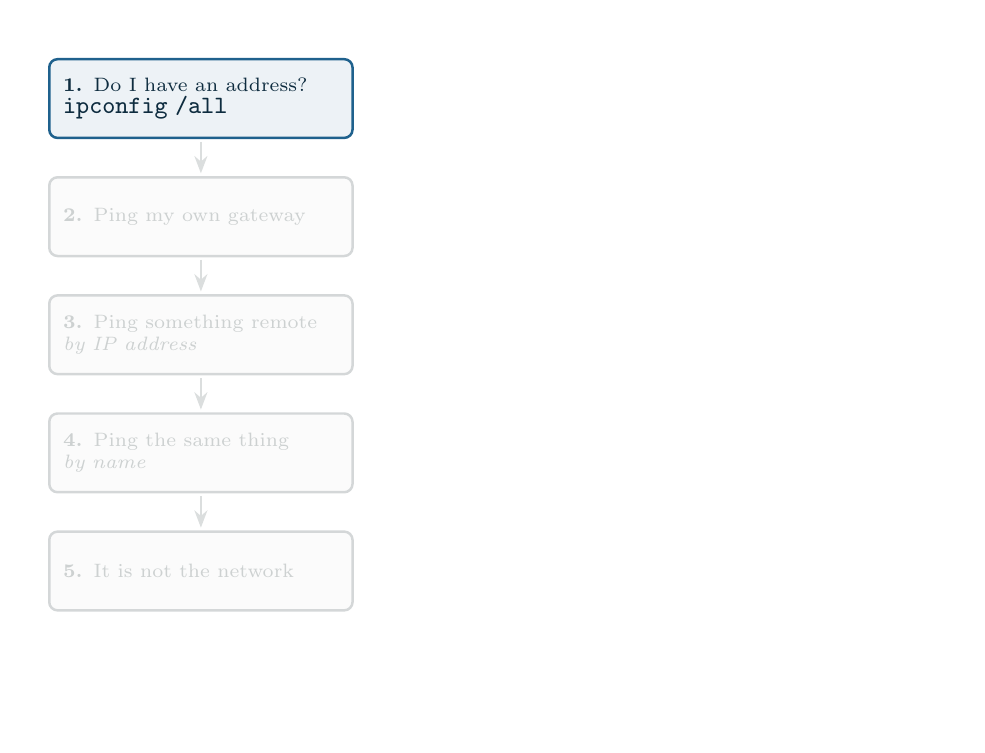
\begin{tikzpicture}[font=\scriptsize]
  \useasboundingbox (-2.2,-7.95) rectangle (9.6,0.9);

  \tikzset{
    rung/.style={rounded corners=3pt, draw=#1, fill=#1!8, text=#1!45!black,
                 line width=0.9pt, text width=3.5cm, align=left,
                 minimum height=1.0cm, font=\scriptsize, inner sep=5pt},
    ghost/.style={rounded corners=3pt, draw=neutral!30, fill=neutral!3,
                  text=neutral!35, line width=0.9pt, text width=3.5cm,
                  align=left, minimum height=1.0cm, font=\scriptsize,
                  inner sep=5pt},
    res/.style={font=\tiny, text=#1!45!black, align=left, anchor=west},
    fl/.style={-{Stealth[length=2.2mm]}, line width=0.9pt, neutral!70},
    stepcap/.style={font=\bfseries, anchor=north west, text width=11.3cm,
                    align=left}}

  % Rung 1 is live from the first beat; 2-5 start as ghosts.
  \node[rung=dom1] at (0,0)
      {\textbf{1.} Do I have an address?\\ \cmd{ipconfig /all}};

  \stepdim{2}{\node[ghost] at (0,-1.5) {\textbf{2.} Ping my own gateway};}
  \stepvis{2}{\node[rung=dom1] at (0,-1.5) {\textbf{2.} Ping my own gateway};}

  \stepdim{3}{\node[ghost] at (0,-3.0)
      {\textbf{3.} Ping something remote\\ \emph{by IP address}};}
  \stepvis{3}{\node[rung=dom1] at (0,-3.0)
      {\textbf{3.} Ping something remote\\ \emph{by IP address}};}

  \stepdim{4}{\node[ghost] at (0,-4.5)
      {\textbf{4.} Ping the same thing\\ \emph{by name}};}
  \stepvis{4}{\node[rung=dom1] at (0,-4.5)
      {\textbf{4.} Ping the same thing\\ \emph{by name}};}

  \stepdim{5}{\node[ghost] at (0,-6.0) {\textbf{5.} It is not the network};}
  \stepvis{5}{\node[rung=dom2] at (0,-6.0)
      {\textbf{5.} It is not the network};}

  % Coordinates, not node names -- the nodes are drawn conditionally, so a
  % \draw naming one would be an undefined-node error at the wrong level.
  \draw[fl, neutral!25] (0,-0.55) -- (0,-0.95);
  \draw[fl, neutral!25] (0,-2.05) -- (0,-2.45);
  \draw[fl, neutral!25] (0,-3.55) -- (0,-3.95);
  \draw[fl, neutral!25] (0,-5.05) -- (0,-5.45);
  \stepvis{2}{\draw[fl] (0,-0.55) -- (0,-0.95);}
  \stepvis{3}{\draw[fl] (0,-2.05) -- (0,-2.45);}
  \stepvis{4}{\draw[fl] (0,-3.55) -- (0,-3.95);}
  \stepvis{5}{\draw[fl] (0,-5.05) -- (0,-5.45);}

  % The verdicts are the payload: each arrives with the rung it belongs to,
  % and unlike the rungs there is no ghost -- an unread verdict would be a
  % spoiler, and the question "so what does it mean if this one fails?" is
  % the one worth asking the room before advancing.
  \stepvis{1}{\node[res=accent] at (2.4,-0.75)
      {fails $\rightarrow$ \textbf{DHCP or layer 2}\\Chapters 20, 14};}
  \stepvis{2}{\node[res=accent] at (2.4,-2.25)
      {fails $\rightarrow$ \textbf{local segment}\\VLAN, cable, ARP,
       wireless assoc.};}
  \stepvis{3}{\node[res=accent] at (2.4,-3.75)
      {fails $\rightarrow$ \textbf{routing, NAT or ACL}\\Chapters 15, 22, 24};}
  \stepvis{4}{\node[res=accent] at (2.4,-5.25)
      {fails $\rightarrow$ \textbf{DNS only}\\Chapter 21};}

  \steponly{1}{\node[stepcap, text=dom1!45!black] at (-2.0,-6.7)
      {Start at the host, not at the core. No address, and nothing else in
       this list can possibly work.};}
  \steponly{2}{\node[stepcap, text=dom1!45!black] at (-2.0,-6.7)
      {The gateway is the last hop still on our own segment. Passing here
       clears the cable, the VLAN and the association.};}
  \steponly{3}{\node[stepcap, text=dom1!45!black] at (-2.0,-6.7)
      {By address, on purpose --- it takes name resolution out of the
       question entirely.};}
  \steponly{4}{\node[stepcap, text=dom1!45!black] at (-2.0,-6.7)
      {Only now bring names back. If 3 passed and 4 fails, exactly one thing
       is left, and it is not the network.};}
  \steponly{5}{\node[stepcap, text=dom2!45!black] at (-2.0,-6.7)
      {Every rung that passes eliminates everything below it. Four commands,
       and the fault is in one of five places.};}
\end{tikzpicture}

\end{document}
